\chapter{Touch panel performance testing (TPPT)}

In touch panel performance testing (TPPT) robot is used to measure the performance of individual touch panels or touch panels integrated to smart devices. Robot performs gestures such as tap and swipe on prescribed positions on the touch panel and the reported coordinates are compared to the accurately known robot coordinates.

Test parameters and test execution are defined by TPPT scripts which are run via TnT UI that provides graphical interface for setting parameters and viewing test progress. Test parameters and results are saved to SQL database (normally SQLite file). The database can then be loaded by TPPT Analysis software which calculates various metrics from the data and presents pass / fail results based on given criteria. Figure \ref{fig:tppt_sw} illustrates the relation between different software components in TPPT.

\begin{figure}[!h]
	\centering
	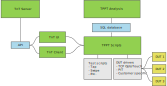
\includegraphics{tppt_sw.pdf}
	\caption{TPPT software overview.}
	\label{fig:tppt_sw}
\end{figure}

\section{TPPT scripts}

TPPT Scripts are Python files that are executed by TnT UI. The UI is used to set script parameters and to control and visualize the script execution.

\subsection{Test script structure}

TnT UI can be used to load and run test scripts. The UI provides an environment where user can give inputs to the test script and the script can easily update its progress, status, indicators etc. It offers a good control over the test scripts.

The scripts define a Context class that is instantiated when the UI loads the scripts. This context consists of all data required to run test cases including TnT Client object, settings, DUT information, tip information, test cases, database session and device driver objects.

Test scripts define a node hierarchy that is visible to the UI as a hierarchy of graphical widgets such as numeric inputs and checkboxes. Each node can define a list of Control objects, which define initial values and valid value ranges for corresponding widgets that are displayed by the UI.

\begin{figure}[!h]
	\centering
	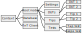
\includegraphics{tppt_node_tree.pdf}
	\caption{TPPT script structure. Each box represents a Python class object.}
	\label{fig:tppt_node_tree}
\end{figure}

The default script implementation divides nodes under Settings, DUTs, Tips and Tests nodes. Each DUT and tip is then also a node under DUTs node and Tips node respectively. Test cases are also defined as nodes under Tests node. The structure is illustrated in Figure \ref{fig:tppt_node_tree}.

Test cases are special TestStep nodes in the sense that they must implement \texttt{execute()} method that is called when the test is to be executed. The test case node class initialization is responsible for defining the controls that show up as widgets in the UI when the script is loaded.

The default script implementation implements \texttt{execute()} method in Context class that loops through all tips, DUTs and test cases that are enabled by the UI. However, utilizing the existing nodes and by writing new ones, it is possible to construct more versatile test sequences that are represented by more complex tree structure.

\subsection{Script context}

Scripts define Context class that stores all necessary data and state for running test sequences. The UI creates an instance of this class when the script is loaded and the class exposes methods for communicating information
between UI and scripts.

Script developer can easily extend and modify the widgets shown in the UI. The parameters member of Context class is a list of key-value pairs that appear in the UI as text input boxes. In the default implementation there are parameters Program, Manufacturer, Version, Operator, Serial and Notes. The values of these parameters are saved to the database.

Script developer can also easily expose button widgets in the UI by adding items to callables member of the Context class. These items are tuples (function, label) where function is a function object defined by script and label is a string used to label the button in UI.

The context object is passed down to test case initialization so that test execution can access the context resources such TnT Client object. Context also exposes indicators member, which can be used by test cases to update test progress in the UI. Indicators basically constitute an HTML element. For a more graphical progress indication, context exposes \texttt{add\_dut\_point(x, y, from\_taplike, expected)} method that can be used by a test case to visualize a touch event and expected points for tap like tests. Expected lines for swipe like tests can be visualized with \texttt{draw\_dut\_expected\_line(start\_x, start\_y, end\_x, end\_y)} method that is also exposed by context.

\subsection{Test case development}

Test cases are nodes in the tree hierarchy. They are classes that inherit the TestStep class. Test case class must define \texttt{execute()} method that is called when test case is executed once sequence is started from the UI and the test case has been enabled. Test case must also implement \texttt{visualize\_grid(dut)} method that returns \texttt{GridVisContainer} object. This method is called when UI is commanded to show points and lines that robot will execute.

Example test case:

\begin{lstlisting}[language=Python]
class MyTestCase(TestStep):

	def __init__(self, context):
		super().__init(“My test case”)
		
		# Show number input field in UI for this test case node
		self.controls.NumPoints = 5
		self.controls.info[“NumPoints”] = {“label”: “Number of points to tap”}

	def execute(self):
		# Add statements to drive robot, collect touch events and save data

	def visualize_grid(self, dut):
		return GridVisContainer(self.__class__.__name__, (dut.width, dut.height), 
		self.create_grid(dut), dut.name)
\end{lstlisting}

\input{from_ui_repo/script.tex}

\section{TPPT analysis}

TPPT Analysis is a standalone application with a web UI. It loads SQL database file produced by execution of TPPT scripts and analyses the results stored therein. Sections below give a detailed description of how to use TPPT Analysis and what kind of results are calculated from the data.

\subsection{Installation}

Installation can be done by running the installation package.

It is required that TPPT scripts are installed before TPPT Analysis can be successfully executed. TPPT Analysis requires configuration file and SQL database file from TPPT script installation.

\subsection{Windows}

The installer is a self-contained exe file which launches a wizard that will help the user through the installation process.

In case the user wants to re-install TPPT Analysis, the following procedure should be followed:
%
\begin{enumerate}
	\item Go to the folder "\tntRootPath" and create a back-up of existing "\tntTPPTAnalysisFolder" folder by renaming the folder as "TPPT Analysis 2020-01-02" where the date is the backup date.
	\item Run installation package as usual (the installer will create a new "\tntTPPTAnalysisFolder" folder).
\end{enumerate}

\subsection{Using TPPT analysis}

\begin{figure}[!h]
	\centering
	\includegraphics[width=12cm]{tppt_analysis_main_view.png}
	\caption{Analysis SW main view.}
	\label{fig:tppt_analysis_main_view}
\end{figure}

To start the analysis software, use shortcut located on desktop or navigate to \texttt{\tntRootPath\tntTPPTAnalysisFolder} and click on the icon named \texttt{\tntTPPTAnalysisExecutable}. This opens a command line prompt and a web browser. The command line prompt shows the status of the application and the browser shows the main view.

\subsubsection{Main view}

The main view is illustrated in Figure \ref{fig:tppt_analysis_main_view}. It shows the test sessions currently in the database and has two different views:
\begin{enumerate}
\item Most recent test sessions (Figure \ref{fig:tppt_analysis_recent_sessions})
\item Hierarchical tree of test sessions (Figure \ref{fig:tppt_analysis_session_hierarchy})
\end{enumerate}

\begin{figure}[!h]
	\centering
	\includegraphics[width=12cm]{tppt_analysis_recent_sessions.png}
	\caption{Most recent test sessions.}
	\label{fig:tppt_analysis_recent_sessions}
\end{figure}

In addition the main view has links to global settings (see Settings view below) and recalculate all –button.

\begin{figure}[!h]
	\centering
	\includegraphics[width=12cm]{tppt_analysis_session_hierarchy.png}
	\caption{Hierarchical view of test sessions.}
	\label{fig:tppt_analysis_session_hierarchy}
\end{figure}

The hierarchical view shows the test sessions categorized by DUT information: Manufacturer name and Program name. The showing of the contents can be toggled by clicking the manufacturer or program name.
If there's incorrect information in the tree, like misspelled manufacturer name, that information can be corrected in DUT settings (see DUT settings view below).

\subsubsection{\label{sec:settings_view}Settings view}

In the settings view the global acceptance limits of the tests can be changed. Changing a test limit results in re-calculation of all test verdicts. 
The settings view can be accessed from the main view under the link 'Settings' as shown in Figure \ref{fig:tppt_analysis_settings_navigation}.

\begin{figure}[!h]
	\centering
	\includegraphics[width=12cm]{tppt_analysis_settings_navigation.png}
	\caption{Settings view navigation.}
	\label{fig:tppt_analysis_settings_navigation}
\end{figure}

The settings are divided to categories based on the tests they are used in ans shown in Figure \ref{fig:tppt_analysis_settings_view}. For each setting the description and the value is shown. The value can be changed by typing a new value to the field. Invalid values are marked with red field background.

\begin{figure}[!h]
	\centering
	\includegraphics[width=12cm]{tppt_analysis_settings_view.png}
	\caption{Settings view.}
	\label{fig:tppt_analysis_settings_view}
\end{figure}

The save button saves the values to the database. At that time all the analysis results are recalculated, which can be a lengthy operation if there are many measurements in the database.

The descriptions of the individual tests are given in sections below starting at Section \ref{sec:one_finger_tap_test}.
Settings should not be changed when there is a test session running. In the worst case it can introduce errors to the TPPT test run.

\begin{figure}[!h]
	\centering
	\includegraphics[width=12cm]{tppt_analysis_recalculate_all.png}
	\caption{Recalculate all.}
	\label{fig:tppt_analysis_recalculate_all}
\end{figure}

The recalculate all button (see Figure \ref{fig:tppt_analysis_recalculate_all}) recalculates all the analysis results in the database. This can take some time if there are many test sessions in the database.

\warningbox{Recalculate all should not be run when there is a test session running. In the worst case it can introduce errors to the TPPT test run and result in incorrect verdicts. If user ends up in this situation, then the results can be recalculated correctly by running Recalculate all when no tests are running.}

\subsubsection{Test session overview}

\begin{figure}[!h]
	\centering
	\includegraphics[width=12cm]{tppt_analysis_session_overview.png}
	\caption{Test session overview.}
	\label{fig:tppt_analysis_session_overview}
\end{figure}

The test session page can be opened by clicking a test session in the main view. The test session view shows the individual test results in a single test run. This is illustrated in Figure \ref{fig:tppt_analysis_session_overview}.
If multiple DUT functionality is enabled, the test results are grouped by DUT. Below the DUT information is link to the DUT settings (see Section \ref{sec:tppt_analysis_test_analysis})

\begin{figure}[!h]
	\centering
	\includegraphics[width=12cm]{tppt_analysis_session_notes.png}
	\caption{Session notes.}
	\label{fig:tppt_analysis_session_notes}
\end{figure}

\begin{figure}[!h]
	\centering
	\includegraphics[width=12cm]{tppt_analysis_session_notes_empty.png}
	\caption{Empty session notes with edit button.}
	\label{fig:tppt_analysis_session_notes_empty}
\end{figure}

At the top of the page the session notes are shown. The first words of the notes are shown also in the main page. The notes can be edited by selecting 'edit', after which the notes can be edited in the text field. The edited notes must be saved by selecting 'save'. Note editing is illustrated in Figures \ref{fig:tppt_analysis_session_notes} and \ref{fig:tppt_analysis_session_notes_empty}.

\subsubsection{DUT settings view}

\begin{figure}[!h]
	\centering
	\subfloat[DUT settings view]{\includegraphics[width=4cm]{tppt_analysis_dut_settings_view.png}\label{fig:tppt_analysis_dut_settings_view}}
	\qquad
	\subfloat[DUT properties and save button]{\includegraphics[width=4cm]{tppt_analysis_dut_properties.png}\label{fig:tppt_analysis_dut_properties}}
	\caption{DUT settings.}
\end{figure}

The DUT settings control the characteristics of the DUT. The settings are separate for each DUT and test session. See Figure \ref{fig:tppt_analysis_dut_settings_view}. The different settings are the following:

\textbf{Touch screen size x}: width of the touch screen in millimeters.

\textbf{Touch screen size y}: height of the touch screen in millimeters.

\textbf{Touch digitizer resolution x}: touch digitizer resolution in direction of width of the screen in pixels.

\textbf{Touch digitizer resolution y}: touch digitizer resolution in direction of height of the screen in pixels.

\textbf{Display native resolution x}: display native resolution in direction of width of the screen in pixels.

\textbf{Display native resolution y}: display native resolution in direction of height of the screen in pixels.

\textbf{Touch screen offset x}: Offset of the actual panel top left from the taught top left corner of the panel in millimeters.

\textbf{Touch screen offset y}: Offset of the actual panel top left from the taught top left corner of the panel in millimeters.

\textbf{Switch X and Y coordinates}: If selected, the X and Y coordinates are exchanged. Switch X and Y-coordinates switch is used before Flip X and Y settings.

\textbf{Flip X coordinates}: Normally the positive X coordinate direction is right. If Flip X coordinates is selected, the direction is reversed (positive direction to left).

\textbf{Flip Y coordinates}: Normally the positive Y coordinate direction is down. If Flip Y coordinates is selected, the direction is reversed (positive direction up).

The Flip X, Flip Y, and Switch X and Y coordinates can be used to adjust to screen rotation. For example, if a typical display is rotated 90 degrees clockwise (positive X direction down, positive Y direction left), this can be adjusted by selecting Switch X and Y coordinates (positive Y direction down, positive X direction left) and Flip X coordinates (positive X direction right).

Below the test session related DUT settings are the DUT properties: Manufacturer name, program name, version, and Sample ID. See Figure \ref{fig:tppt_analysis_dut_properties}.

All the settings are saved by pressing 'Save all'. After the settings have been changed, the measurements in the test session are re-calculated to accommodate new settings.

\subsubsection{Test session summary}

Summary page lists all results of tests run in test session. Test session overview is in the top of the page. From each test item the general test results are shown. In order to view the detailed results, click the corresponding table row to open the full test report.

\warningbox{Test case verdict is calculated and stored to the database when test report is opened. If the test is still running, the verdict may be incorrect. This can be fixed by opening the test report again after the test is finished and the verdict can be correctly determined.}

\subsection{\label{sec:tppt_analysis_test_analysis}Common items in test reports}

\begin{figure}[!h]
	\centering
	\includegraphics[width=10cm]{tppt_analysis_common_items.png}
	\caption{Common items.}
	\label{fig:tppt_analysis_common_items}
\end{figure}

At the top of the test report page are the functions common to all test reports (see Figure \ref{fig:tppt_analysis_common_items}):

\textbf{Back}: Return to test session view.

\textbf{Analysis Home}: Return to main page

\textbf{Print}: Print the test report. 

\textbf{Load CSV}: Load the test item raw data as a CSV file.

\textbf{Note}: Use the print button in the test page rather than the browser’s print function. The print button is disabled when all the images in the report are not yet loaded.

When detailed plots (pictures) are shown in test reports, they can be toggled by the toggle buttons (see Figure \ref{fig:tppt_analysis_toggle_buttons}):

\begin{figure}[!h]
	\centering
	\includegraphics[width=10cm]{tppt_analysis_toggle_buttons.png}
	\caption{Toggle buttons.}
	\label{fig:tppt_analysis_toggle_buttons}
\end{figure}

\textbf{All}: Toggles the state of all detailed plots.

\textbf{Failed}: Toggles the state of failed plots

\textbf{Passed}: Toggles the state of passed plots

If some of the plots are manually opened and then toggle button is pressed, the plots are all either opened or closed, depending on the state of the detailed plots. The desired state can be achieved with at most two presses of the toggle button.

\subsection{\label{sec:one_finger_tap_test}One Finger Tap Test}

One Finger Tap Test report shows the results of the tap test. The tap test is used to measure the tap accuracy performance of the DUT.

\subsubsection{Settings}

The settings (see Section \ref{sec:settings_view}) related to the one finger tap test are:

\textbf{Maximum allowed positional error}: The distance from the point that the robot presses to the coordinates reported by the DUT.

\textbf{Maximum allowed missing inputs}: The maximum allowed amount of missing inputs in the test.

\textbf{Edge area distance from edge in Tap test}: The edge area width. The edge area can have different thresholds than rest of the DUT. If this setting is positive (larger than 0), the edge area analysis is enabled and the two following settings are in use:

\begin{enumerate}
\item \textbf{Maximum allowed positional error in edge area}: The maximum allowed positional error if the point that the robot presses resides in the edge area.
\item \textbf{Maximum allowed missing edge inputs}: The maximum allowed amount of missing inputs in the edge area in addition to the global value. Thus, if the global value is 1 and missing edge inputs value is 2, there can be at most 3 missing inputs in the edge area if none are missing in other parts of the DUT.
\end{enumerate}

\subsubsection{Report contents}

The detailed results are:

\textbf{Max accuracy error: Maximum accuracy error}. If edge area analysis is enabled, this is reported for both the edge area and for the rest of the display (center).

\textbf{Missing inputs}: Missing inputs in the test. If edge area analysis is in use, this is reported separately for the edge area and for the rest of the display (center).

\subsubsection{Preview images}

The first preview image illustrated in Figure \ref{fig:tppt_analysis_tap_preview} shows the overview of the DUT. Circles represent the robot points and the size of the circle is the size of the allowed area given by accuracy error. If the input is missing, the circle is drawn red. If the input is outside the allowed area, the position of the input is shown with red marker, otherwise a green marker is used.

\begin{figure}[!h]
	\subfloat[Preview]{\includegraphics[width=8cm]{tppt_analysis_tap_preview.png}\label{fig:tppt_analysis_tap_preview}}
	\subfloat[Scatter plot]{\includegraphics[width=8cm]{tppt_analysis_tap_scatter.png}\label{fig:tppt_analysis_tap_scatter}}
	\caption{Tap test.}
\end{figure}

The second image illustrated in Figure \ref{fig:tppt_analysis_tap_scatter} gives the scatter plot. It plots all the measurements in relation with the point that the robot has pressed (reference point). In the image the distribution of the tap error can be observed. The histograms on the sides show the distribution of the points on the axes. The unit in the histogram is one measured event, and the cumulative amount of events in each bar can be read from the scale of the respective histogram. If edge analysis is conducted, two acceptance circles are shown (see above).

The last image(s) give the same scatter information with limited display area. This is useful if there are erroneous measurements that are far from the reference point. With limited display area the points near the reference point can be viewed in more detail.

All the preview images can be viewed in higher resolution by clicking the preview image.

\subsection{One Finger Swipe Test}

The one finger swipe test report shows the results of the swipe test. The swipe test is used to measure the accuracy of the DUT, when the touch is in linear motion.

\subsubsection{Settings}

\begin{figure}[!h]
	\centering
	\includegraphics[width=14cm]{tppt_analysis_swipe_parameters.png}
	\caption{Swipe parameters.}
	\label{fig:tppt_analysis_swipe_parameters}
\end{figure}

The settings related to the one finger swipe test are:

\textbf{Maximum allowed offset}: The maximum allowed offset of swipe point perpendicular to the line that the robot has swiped (see Figure \ref{fig:tppt_analysis_swipe_parameters}). 

\textbf{Maximum allowed jitter}: Maximum allowed jitter in a swipe. Jitter is the peak-to-peak maximum movement perpendicular to the swipe line within a sliding window (see Figure \ref{fig:tppt_analysis_swipe_parameters} above). 

\textbf{Jitter search mask}: The width of window in mm along the swipe line in which the jitter is calculated. 

\textbf{Maximum amount of missing swipes}: A swipe is missing if no points are reported for a single swipe. If the number of missing swipes is more than the maximum amount, the test has failed.

\subsubsection{Report contents}

\begin{figure}[!h]
	\centering
	\includegraphics[width=10cm]{tppt_analysis_swipe_summary.png}
	\caption{Swipe test summary tables.}
	\label{fig:tppt_analysis_swipe_summary}
\end{figure}

The report shows the maximum offset measured in the test, maximum jitter and the amount of missing swipes. The summary table is shown in Figure \ref{fig:tppt_analysis_swipe_summary}. If these values are within configured limits, they are marked Pass. Total test verdict is Pass is all of these results are Pass. If any of them is Fail then test verdict is Fail. It is possible that maximum jitter or maximum offset are 'N/A' if there is insufficient data (less than two points per swipe). If either one is 'N/A', the test case verdict is 'N/A' if the number of missing swipes is less than the maximum allowed missing swipes. If there are more swipes missing than allowed, the test verdict is Fail regardless of jitter and offset verdicts.

Below the summary table in Figure \ref{fig:tppt_analysis_swipe_summary} there is another table showing the maximum deviation from fitted lines and the mean of maximum deviations from each fitted line. These two values don't have a verdict and hence don't directly affect the total test case verdict.

\subsubsection{Preview images}

\begin{figure}[!h]
	\centering
	\includegraphics[width=10cm]{tppt_analysis_swipe_preview.png}
	\caption{Main swipe test preview image.}
	\label{fig:tppt_analysis_swipe_preview}
\end{figure}

The main preview image illustrated in Figure \ref{fig:tppt_analysis_swipe_preview} shows the swipes and the measured points. The swipes are shown with gray arrows. The measured points are colored green or red based on their offset values – the values exceeding the maximum allowed offset are colored red. If maximum allowed jitter is exceeded, it is not shown on the preview image. A higher resolution version of the image is available by clicking the preview image on the report.

\begin{figure}[!h]
	\centering
	\includegraphics[width=10cm]{tppt_analysis_swipe_details.png}
	\caption{Swipe details.}
	\label{fig:tppt_analysis_swipe_details}
\end{figure}

In Figure \ref{fig:tppt_analysis_swipe_details} the detail table shows the maximum offset and jitter values for each individual swipe. The Pass / Fail value of a swipe is determined by the offset and jitter values and whether the swipe is missing. A swipe is missing if it has no measurement points. If a swipe has at least one point, it is not considered missing.

If the maximum offset within a swipe exceeds the configured limit, the individual swipe is Fail and also the total test verdict is Fail. If a swipe has no measurement points, the swipe offset verdict is 'N/A'. Value 'N/A' does not affect the maximum offset verdict of the entire test case, but it is treated as missing swipe.

If the maximum jitter within a swipe exceeds the configured limit, the individual swipe is Fail and also the total test verdict is Fail. If a swipe has less than two measurement values, the jitter value is 'N/A', as jitter calculation requires at least two measurement values. Value 'N/A' does not affect the maximum jitter verdict of the entire test case.

If a swipe is missing, the verdict of the individual swipe is Fail but the total test case verdict may still be Pass if the number of missing swipes does not exceed the configured limit and also offset and jitter are within limits. Hence it is possible that a test case with verdict Pass has individual swipes with verdict Fail.

The individual swipe plot images illustrated in Figure \ref{fig:tppt_analysis_swipe_details} show the measured swipe points on the left and the detailed analysis of the swipe on the right. The detailed analysis shows the offset for each point (blue) and the calculated jitter (red). The x-axis is measured along the robot swipe line. Vertical lines (gray) show the location of the measurement point in the X axis. 

\subsection{One Finger Stationary Jitter Test}

One finger stationary jitter report reports the results of the stationary jitter test. It is used to test the performance of the DUT when a single point is pressed and hold. Optimally the DUT should report a single coordinate consistently.

\subsubsection{Settings}

The one finger stationary jitter test has the following settings:

\textbf{Maximum allowed stationary jitter}: The maximum amount of jitter allowed for a single point.

\subsubsection{Report contents}

The stationary jitter reports the maximum measured stationary jitter in the test. In addition, the results for individual points pressed are measured.

The jitter is calculated from the first coordinate reported by the DUT. The jitter for each successive measurement value is the distance from the first reported point. The jitter reported for an individual tap is the maximum of jitters for individual points.

\subsubsection{Preview images}

\begin{figure}[!h]
	\centering
	\includegraphics[width=10cm]{tppt_analysis_stationary_jitter_details.png}
	\caption{Stationary jitter details.}
	\label{fig:tppt_analysis_stationary_jitter_details}
\end{figure}

The main preview image illustrated in Figure \ref{fig:tppt_analysis_stationary_jitter_details} shows the different points measured related to the DUT. Passed points (jitter value not exceeding threshold) are marked green, failed points are marked with red color. Note that the passed points are determined by the first input from the panel – the analysis does not take robot touch point into account when determining the pass/failure limits.

\subsection{One Finger Tap Repeatability Test}

The one finger tap repeatability report shows the results of the repeatability test. The tap repeatability test is used to measure the panel’s ability to report consistent coordinates when the same location of the panel is pressed repeatedly with the robot.

\subsubsection{Settings}

The settings related to the tap repeatability test are:

\textbf{Maximum tap repeatability error}: The maximum distance of the reported points either in x- or y-direction.

\subsubsection{Report contents}

The report shows the maximum repeatability errors in both x- and y-directions. The maximum errors reported may be from different measurement points. 

Individual measurement points are reported in a table with respective errors in x- and y-directions.

\subsubsection{Preview images}

The main preview image shows the passed and failed points located in the DUT. The point is passed if errors in both the x- and y-directions are less than equal to the maximum repeatability error.

\begin{figure}[!h]
	\centering
	\includegraphics[width=10cm]{tppt_analysis_tap_repeatability_details.png}
	\caption{One finger tap repeatability details.}
	\label{fig:tppt_analysis_tap_repeatability_details}
\end{figure}

The detailed images illustrated in Figure \ref{fig:tppt_analysis_tap_repeatability_details} show the location of the taps. The reference point shows the location that the robot has tapped. The inner box in the image shows the acceptance area of the measurements. The measurements outside the acceptance area are marked failed with red color. 

Note: the acceptance area is not an absolute definition, it is estimated from the measurement values. The pass/fail value is absolute, as it is calculated from peak-to-peak values of the measurements in both x- and y-directions.

\subsection{One Finger Stationary Reporting Rate Test}

The one finger stationary reporting rate test reports the results of the stationary reporting rate test. It measures the reporting frequency of the DUT.

Note: This test is platform-specific. Some platforms, like Android, do not report tap events if the tap is stationary. In those platforms the stationary reporting rate test is not applicable.

\subsubsection{Settings}

The settings related to the stationary reporting rate test are:

\textbf{Minimum allowed reporting rate}: The minimum reporting rate that is allowed. Measured in Herz (Hz).

\subsubsection{Report contents}

The report contains the minimum measured reporting rate for the test. The reporting rate is calculated from time intervals between reported coordinates from DUT. 

The detailed table shows the measured minimum and maximum reporting rate for each measured point. 

\subsubsection{Preview images}

The main preview image shows the measured points on the DUT, and marks the point passed (green) or failed (red) based on the minimum reporting rate for that specific point.

\begin{figure}[!h]
	\centering
	\includegraphics[width=10cm]{tppt_analysis_stationary_reporting_rate_details.png}
	\caption{Stationary reporting rate details.}
	\label{fig:tppt_analysis_stationary_reporting_rate_details}
\end{figure}

The detailed image illustrated in Figure \ref{fig:tppt_analysis_stationary_reporting_rate_details} shows the reporting rate for an individual tap. The X axis is the DUT event index, and the Y axis shows the delay from the previous event. The red line (if visible) shows the acceptance limit. Delays above the acceptance limit are considered failed. Note: the acceptance limit is the reciprocal of the minimum allowed reporting rate.

\subsection{One Finger Non-Stationary Reporting Rate Test}

The One finger non-stationary reporting rate test report shows the results for non-stationary reporting rate test.

Note: the applicability concerns for stationary reporting rate test do not apply for non-stationary reporting rate test.

\subsubsection{Settings}

The settings related to the stationary reporting rate test are:

\textbf{Minimum allowed reporting rate}: The minimum reporting rate that is allowed. Measured in Herz (Hz).

\subsubsection{Report contents}

The report contains the minimum measured reporting rate for the test. The reporting rate is calculated from time intervals between reported coordinates from DUT. Additionally the amount of missing lines (missing inputs) is reported.

The detailed table shows the measured minimum and maximum reporting rate for each measured point. 

\subsubsection{Preview images}

\begin{figure}[!h]
	\centering
	\includegraphics[width=10cm]{tppt_analysis_non_stationary_reporting_rate_preview.png}
	\caption{Non-stationary reporting rate preview.}
	\label{fig:tppt_analysis_non_stationary_reporting_rate_preview}
\end{figure}

The main preview image illustrated in Figure \ref{fig:tppt_analysis_non_stationary_reporting_rate_preview} shows the measured points on the DUT, and marks the point passed (green) or failed (red) based on the minimum reporting rate for that specific point. The arrows show the location and direction of robot movement.

The detailed preview image is the same than in stationary reporting rate test (see above).

\subsection{Two Finger Separation Test}

The separation test report shows the results for the separation test that is used to measure the DUTs ability to separate distinct fingers (effectors) based on their distance from each other.

\subsubsection{Settings}

The settings related to the separation test are:

\textbf{Maximum allowed finger separation distance (vertical and horizontal)}: The maximum distance in which the fingers are allowed to be interpreted as one input. If the DUT cannot detect distinct fingers with larger separation distances than the setting, the result is fail. This setting is used for horizontal and vertical finger alignments.

\textbf{Maximum allowed finger separation distance (diagonal)}: The maximum distance in which the fingers are allowed to be interpreted as one input in other directions than strictly horizontal or vertical.

\subsubsection{Report contents}

The first table lists the measured separation distances with the different separation angles. The distance measured is the first distance with which the different fingers are detected as separate fingers and all the successive tests with larger separation distances are also successful.

If the separation distance is larger than the maximum allowed setting for that angle, the measurement is marked as failed.

In the second table, all the different measurements with all angles and separation distances are listed. Individual measurement is marked as passed, if the different fingers could be detected. If an individual test fails with separation distance less or equal to maximum allowed setting, the failed test does not affect the overall result of the test.

\subsubsection{Preview images}

\begin{figure}[!h]
	\subfloat[Preview]{\includegraphics[width=8cm]{tppt_analysis_separation_preview.png}\label{fig:tppt_analysis_separation_preview}}
	\subfloat[Details]{\includegraphics[width=8cm]{tppt_analysis_separation_details.png}\label{fig:tppt_analysis_separation_details}}
	\caption{Separation test.}
\end{figure}

The first preview image of the separation test illustrated in Figure \ref {fig:tppt_analysis_separation_preview} shows the overall results for the test. It shows the individual robot positions, in which the fingers have been pressed. Each position is marked as passed or failed depending on the individual separation result.

The second image illustrated in Figure \ref{fig:tppt_analysis_separation_details} shows the analysis of the test results based on the actual detected finger events. The event positions detected as separate are marked with green color. The event positions that show only one finger id (fingers are detected as one), are marked with red color.

\begin{figure}[!h]
	\centering
	\includegraphics[width=10cm]{tppt_analysis_separation_details_2.png}
	\caption{Separation test details.}
	\label{fig:tppt_analysis_separation_details_2}
\end{figure}

The details image illustrated in Figure \ref{fig:tppt_analysis_separation_details_2} shows the received events from a single separation test with single angle and separation distance. The events are marked to the picture with red or green markers. The events having the same event id are connected by solid lines. The finger positions of the robot are marked with circles.

\subsection{Multifinger Tap Test}

Multifinger Tap Test report shows the results of the multifinger tap test. The multifinger tap test is used to measure the tap accuracy performance of the DUT when the DUT is operated with multiple fingers.

\subsubsection{Settings}

The settings related to the multifinger tap test are:

\textbf{Maximum allowed positional error}: The distance from the point that the robot presses to the coordinates reported by the DUT.

\textbf{Maximum allowed missing inputs}: The maximum allowed amount of missing inputs in the test.

Note: the edge area analysis is not supported in the current version of analysis software.

\subsubsection{Report contents}

The detailed results are:

\textbf{Max accuracy error}: Maximum accuracy error. 

\textbf{Missing inputs}: Missing inputs in the test. 

\textbf{Errors}: The errors detected while analyzing the images.

The detailed results table shows the results for individual taps. For each tap the number of fingers, errors, and maximum offset are reported. The individual test fails if the maximum offset is exceeded or there are errors in the test.

\subsubsection{Preview images}

\begin{figure}[!h]
	\subfloat[Preview]{\includegraphics[width=8cm]{tppt_analysis_multifinger_tap_preview.png}\label{fig:tppt_analysis_multifinger_tap_preview}}
	\subfloat[Details]{\includegraphics[width=8cm]{tppt_analysis_multifinger_tap_details.png}\label{fig:tppt_analysis_multifinger_tap_details}}
	\caption{Multifinger tap test.}
\end{figure}

The overview image illustrated in Figure \ref{fig:tppt_analysis_multifinger_tap_preview} shows the passed and failed mesurements on the DUT. Only the location of the first finger is reported. Thus, each point on the DUT corresponds to one tap with multifinger effector.

The detailed overview image illustrated in Figure \ref{fig:tppt_analysis_multifinger_tap_details} is similar to the overview image, but it shows additionally the all the fingers in the multifinger effector connected by a line. If the effector lines overlap, the resulting image may be difficult to interpret (see above). In these cases the detailed locations of the effector can be seen in the detailed images (see below).

\begin{figure}[!h]
	\subfloat[Scatter plot]{\includegraphics[width=8cm]{tppt_analysis_multifinger_tap_scatter.png}\label{fig:tppt_analysis_multifinger_tap_scatter}}
	\subfloat[Details]{\includegraphics[width=8cm]{tppt_analysis_multifinger_tap_details_2.png}\label{fig:tppt_analysis_multifinger_tap_details_2}}
	\caption{Multifinger tap test details.}
\end{figure}

The scatter plot illustrated in Figure \ref{fig:tppt_analysis_multifinger_tap_scatter} shows the tap locations for each of the taps and in each of the effector fingers. Only a limited version is shown, as the errors in the tap test quickly render the scatter plot non-usable.

The tap details image illustrated in Figure \ref{fig:tppt_analysis_multifinger_tap_details_2} shows one tap with multifinger effector along with the measured events from the DUT. The upper portion of the image shows the general results of the tap. The circles give the maximum position error related to the effector positions. If a point is failed, a red line connects the point to the effector position (see above). 

The small scatter diagrams show the individual finger results of the effector. For each finger, the amount of events is reported (n, e.g. for Finger 1 the amount of events is 100) and the finger id received in the event. 

Note: the finger ids can be used to detect errors. Generally the finger ids are distributed randomly between different effector fingers, but there should always be exactly one finger id per effector finger.

\subsection{Multifinger Swipe Test}

The multifinger swipe test report shows the results for the multifinger swipe test that is used to measure the performance of the DUT when it is used with multiple fingers in a swiping motion.

\subsubsection{Settings}

The settings related to the multifinger swipe test are:

\textbf{Maximum allowed offset}: The maximum allowed offset of swipe point perpendicular to the line that the robot has swiped (see Figure \ref{fig:tppt_analysis_swipe_parameters} above). 

\textbf{Maximum allowed jitter}: Maximum allowed jitter in a swipe. Jitter is the peak-to-peak maximum movement perpendicular to the swipe line (see Figure \ref{fig:tppt_analysis_swipe_parameters} above). 

\textbf{Jitter search mask}: The distance (or window) along the swipe line in which the jitter is calculated. 

\textbf{Maximum amount of missing swipes}: A swipe is missing if no points are reported for a single swipe. If the number of missing swipes is more than the maximum amount, the test has failed.

The values are the same than in the one finger swipe test.

\subsubsection{Report contents}

The first table reports the maximum offset and jitter in any of the swipes and the number of missing swipes. Additionally, the possible errors in the analysis are reported.

The detailed table gives the offset and jitter for each of the individual multifinger swipes.

\subsubsection{Preview images}

\begin{figure}[!h]
	\centering
	\includegraphics[width=10cm]{tppt_analysis_multifinger_swipe_preview.png}
	\caption{Multifinger swipe test preview.}
	\label{fig:tppt_analysis_multifinger_swipe_preview}
\end{figure}

The first preview image illustrated in Figure \ref{fig:tppt_analysis_multifinger_swipe_preview} shows the multifinger swipes on the DUT. All the swipes and all the fingers are plotted. The received events are shown with markers, green (passed) and red (failed) depending on the offset value of the event. The robot swipes are shown with arrows (hidden behind the markers in the example figure above).

\begin{figure}[!h]
	\centering
	\includegraphics[width=10cm]{tppt_analysis_multifinger_swipe_details.png}
	\caption{Multifinger swipe test details.}
	\label{fig:tppt_analysis_multifinger_swipe_details}
\end{figure}

The multifinger swipe details image illustrated in Figure \ref{fig:tppt_analysis_multifinger_swipe_details} gives the same information than the one finger swipe details image, but each of the fingers are plotted separately. For each of the fingers, the number of measurements and finger id received in the event is plotted.
